\subsection{Design}

\subsubsection{Introduction}

This section discusses the design of the web-based version of the application.
The design of the application was constructed with only the most important
functional and non-functional requirements in mind. The web-based version was
classed as an optional extension of the project, with preliminary effort
directed solely towards the desktop application.

\subsubsection{Terminology}

The web application design and implementation section discusses many
web technologies along with their acronyms. The acronyms will be
described with a brief overview of the technology.

\begin{itemize}
\item HTML: Hyper Text Markup Language. HTML is the basis of every web page
structure. It is a structured document with tags denoted by angle brackets (such
as $<$html$>$). These tags form a nested, tree-like structure that is read by 
the browser to create the page layout of the website.
\item CSS: Cascading Style Sheets. CSS provides the style information for the
HTML document. CSS enables the separation of the HTML document content from the
document's presentation and defines a consistent approach for specifying the 
style of an HTML document.
\item JS: JavaScript. JS is an interpreted computer programming language used by
browsers to provide dynamic, interactive web page content without requiring
communication with the web server. JS is bundled alongside an HTML document.
\item jQuery and jQuery UI: These are libraries (bundles) of JavaScript code to
simplify the development of JavaScript.
\item PHP: PHP Hypertext Preprocessor. PHP is a server-side computer programming
language used to generate dynamic web pages prior to sending the web page on to 
the browser in the form of HTML. PHP may interact with databases and other 
external data sources during the creation of the web page.
\item SQL: Structured Query Language. A high-level language for expressing what
a user wants from a database.
\item MySQL. The relational database management system that manages some data 
set represented by tables. MySQL also accepts SQL queries and will return data 
that matches what the SQL query requests.
\end{itemize}

This report discusses graph theory and network flow relating to the
Ford-Fulkerson algorithm in significant depth. This is discussed in a separate
section, section \ref{sec:graphTheoryAndNetworkFlow}.

\subsubsection{System architecture}

The web application is a standard multi-tier architecture with the 
presentation, logic, and data separated from each other.

The presentation tier is the client/browser who has Hyper Text Mark-up Language
(HTML) and Cascading Style Sheets (CSS) for the static presentation of content.
In addition there is JavaScript supported by JQuery and JQueryUI for the dynamic
user interface elements.

The logic tier runs on a web server called Lighttpd (pronounced lighty) that is
supported by PHP: Hypertext Preprocessor (PHP). The logic tier has two data
sources that make up the data tier, a MySQL database containing the latest data
and a Java jar for looking back at older data.

The specific server-side technologies were chosen for two reasons. One member
of the team had working knowledge of setting up and maintaining the systems and
also there was a discussion on having the web application hosted by the
University. The University's servers have PHP and MySQL installed meaning a
port of the web application, if one had been required, would have been trivial.
With the web application running fine on a third-party Virtual Private Server
this was deemed unnecessary.

The N-Tier Architecture diagram is available from appendix
\ref{fig:nTierArchitecture}.

\subsubsection{User interface}

The user interface of the web application was intended on being as close to the
desktop interface as viable within the constraints of a web browser and within
the realms of what is a typical layout of a web page.

A wireframe for the web application is shown in appendix
\ref{fig:webApplicationWireframe}.

A screenshot of the final design is shown in Figure~\ref{fig:webAppScreenshot}.

\begin{figure}
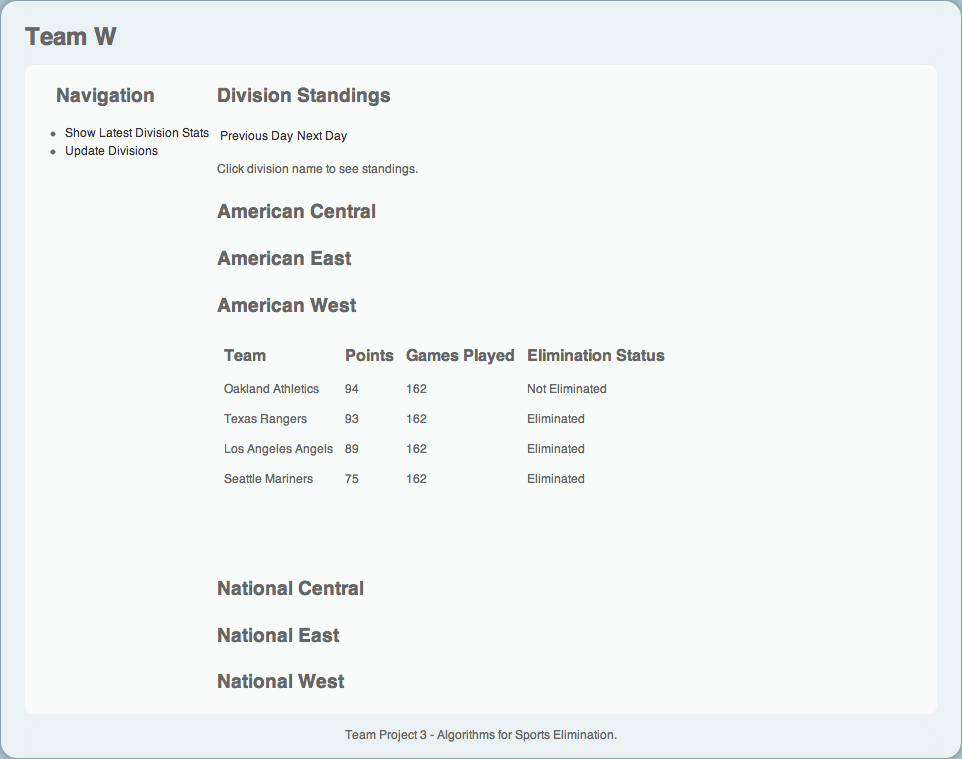
\includegraphics[width=\linewidth,keepaspectratio]
{images/webAppScreenshot.png}
\caption{Web Application Screenshot}
\label{fig:webAppScreenshot}
\end{figure}

The web application has a single page containing the six available divisions.
Each division is a table and only one is available for viewing at a time. The 
reasoning behind this is to keep as much information `above the fold' (above the
lower page boundary on a browser's window).

There are links at the top of each page that will allow the user to traverse
the entire date range for the season allowing them to view the scoreboard and
elimination status at any point in time.

\subsection{Implementation}

\subsubsection{Introduction}

This section discusses the implementation of the web-based version of the
application. The implementation discussion will be split up into the three
main sections as shown in appendix~\ref{fig:nTierArchitecture}.

\subsubsection{Presentation - Client/Browser}

The website uses three of the most common web technologies in use: HTML, CSS,
and JavaScript (supported by jQuery and jQuery UI).

The layout of the HTML and related CSS presentation have been designed to be
as simple and easy to look at as possible. A soft colour palette is used to
prevent flashy content from distracting any use from the content. There is
a small navigation section on the left hand side that contains a couple of
links, one for showing the latest division statistics, and one to update
the divisions. The latter would not be required in a production system with
automatic updates.

The layout is supported with JavaScript with supporting libraries jQuery and
jQuery UI. This allowed an effect known as `accordion' to be implemented. This
enables hidden content sections that only show a header, in this case the
division names. When the division name is clicked that division's table is
shown. Just like in the desktop user interface, only one division can be viewed
at one time. This provides a similar interface and prevents content from
making the page very long requiring the user to scroll to find their
favourite division.

There are two links, `Previous Day' and `Next Day', that allow the user to
see how teams were doing during previous dates in the league with a quick
link at the side (as mentioned previously) back to the most recent results.

\subsubsection{Logic - Web Server/PHP Processor}

The website is dynamically created by using PHP. PHP interfaces with 
the data layer sections and, from the results obtained from the data layer,
produces the division tables and pushes the generated HTML along with the
attached CSS and JavaScript.

Based on two URL variables, one representing the page requested, and another
the date, the PHP script makes appropriate calls to the MySQL or Java JAR data
stores. The PHP script also increments and decrements the date requested (if
applicable) and presents these are previous and next links to the user to allow
them to see their favourite division's league status during previous days
during season.

\subsubsection{Data}

The web application has two primary sources of data: a MySQL database and a
Java JAR file. The MySQL database contains the recent information available
on the sports divisions whereas the Java JAR contains a text file of the entire
result set allowing the user to request to see the state of a division at any
point in the league.

\subsubsection{Data - MySQL Database}

The database is structured with six tables, one for each division. Each table
structure is identical with columns for the team name, the number of points
a team has, the number of games they have played, and whether or not they have
been eliminated from the division. This allows for a direct mapping from
database storage to the user's view. The structure also greatly simplified 
database queries as information from an entire division was a single simple, and 
thus efficient, SQL query. An example query to see the league table, ordered by 
number of points for the American West division is shown below:

\begin{verbatim}
SELECT *
FROM `American West`
ORDER BY Points DESC;
\end{verbatim}

This database is updated with the latest division statistics supplied by the 
Java JAR as the JAR contains the algorithm to compute the elimination status.
The update can be completed in two ways. If the division is new and thus no
information is present in the table an INSERT INTO statement is performed for
each time. If the team is present within the database (as found via a SELECT
statement), an UPDATE is completed instead. Examples of the three queries
for the American West division team `Los Angeles Angels' are shown below:

\begin{verbatim}
SELECT *
FROM `American West`
WHERE Team = `Los Angeles Angels';
\end{verbatim}

\begin{verbatim}
INSERT INTO `American West`
       (Team, Points, `Games Played`, Eliminated)
VALUES (`Los Angeles Angels`, 89, 162, 1);
\end{verbatim}

\begin{verbatim}
UPDATE `American West`
SET Points = 89,
    `Games Played` = 162,
    Eliminated = 1
WHERE Team = `Los Angeles Angels`;
\end{verbatim}

\subsubsection{Data - Java JAR}

The JAR file has embedded within it a text file containing the entire list of
results from every match in the baseball season being discussed. This is parsed
on-demand up to the date specified by the user. This allows users to ask to see 
the results and associated elimination status at any point in time. This is
called by the PHP script using the URL variable `date'. An example URL and
the associated command line call are below.

\begin{verbatim}
gordonrenfrewshire.com/teamw/index.php?page=showDivisions&date=4-10-2012
\end{verbatim}

\begin{verbatim}
java -jar elim.jar --web 4-10-2012
\end{verbatim}

This is not 
the most efficient method of implementation however the web application as a 
whole was an extension to the primary aims of the project and as a result wasn't 
started until the second semester after the desktop application had been 
significantly implemented. With the time constraints and significant complexity 
of a more efficient implementation it was decided that this was the best 
solution with the current resources. A more efficient implementation was 
assigned to the future work section of the project.


